Når vi har sett på transistorer har vi sett på de 3 terminalene Base, Collector
og Emitter.
For helligdom og mystikk kalles de i FET-sammenheng for Gate, Drain og Source.
\\\\
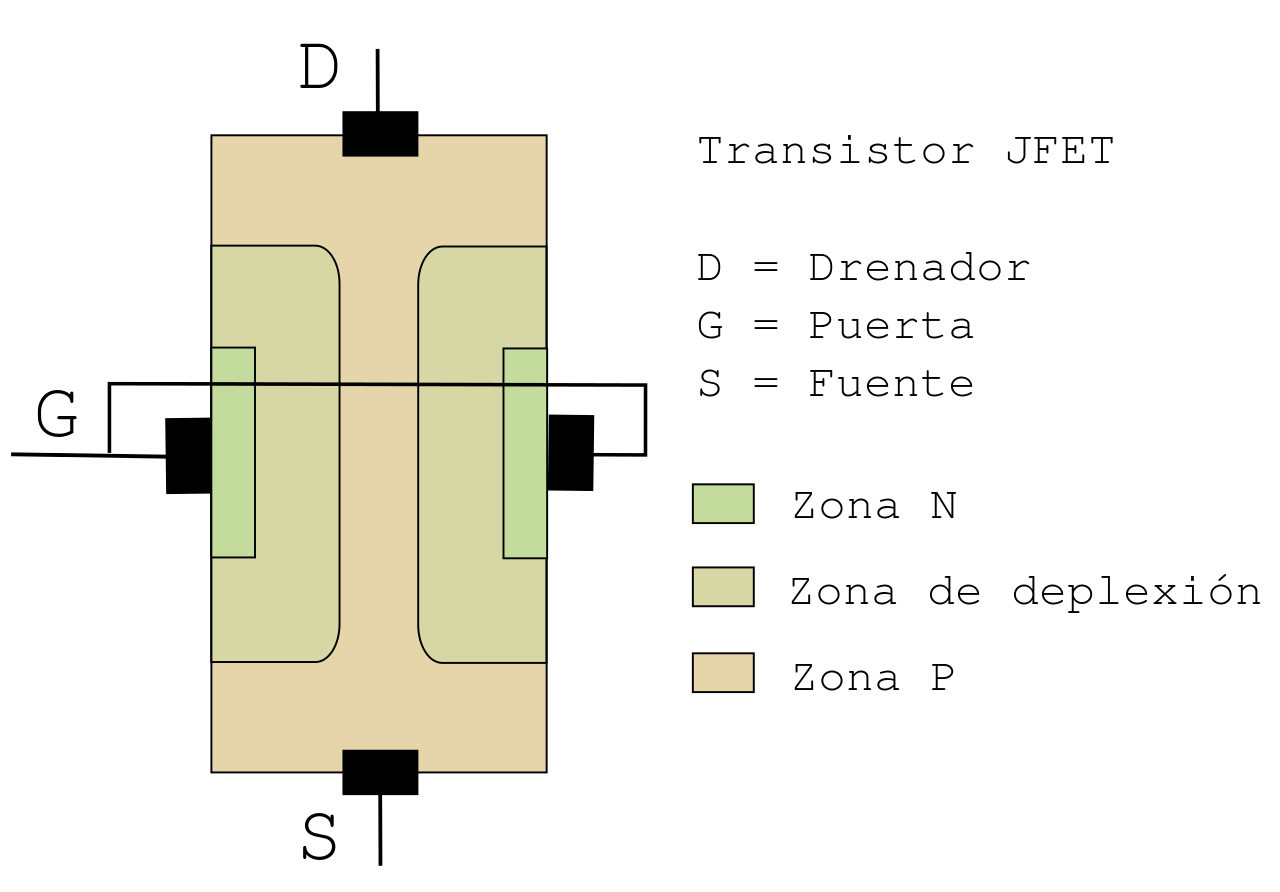
\includegraphics[width=\textwidth]{./img/jfet}
\\\\
Gate er koblet på n-dopet materiale, vi ser sperresjikte i lysegrønn og
i midten er et p-dopet materiale.
Dette bildet er et eksempel på p-channel JFET.
Hvis n og p materialene var byttet om ville det være en n-channel.
